\definecolor{tblue}{RGB}{61,142,221}
\definecolor{torange}{RGB}{253,143,41}
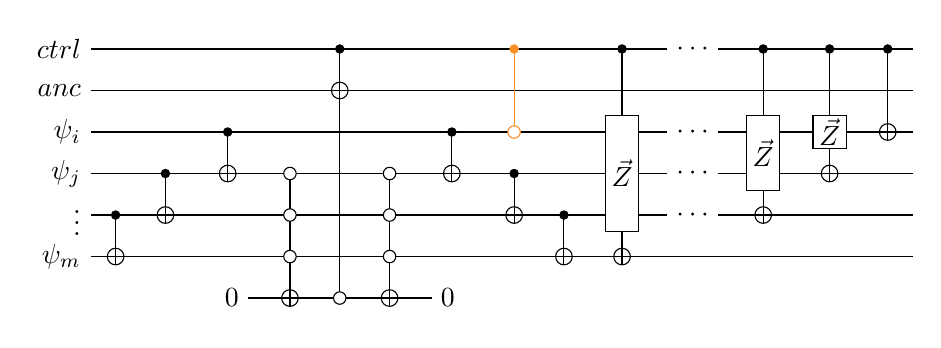
\begin{tikzpicture}[scale=1.000000,x=1pt,y=1pt]
\filldraw[color=white] (0.000000, -7.500000) rectangle (297.000000, 97.500000);
% Drawing wires
% Line 4: ctrl W ctrl
\draw[color=black] (0.000000,90.000000) -- (297.000000,90.000000);
\draw[color=black] (0.000000,90.000000) node[left] {$ctrl$};
% Line 5: anc W anc
\draw[color=black] (0.000000,75.000000) -- (297.000000,75.000000);
\draw[color=black] (0.000000,75.000000) node[left] {$anc$};
% Line 6: i W \psi_i
\draw[color=black] (0.000000,60.000000) -- (297.000000,60.000000);
\draw[color=black] (0.000000,60.000000) node[left] {$\psi_i$};
% Line 7: j W \psi_j
\draw[color=black] (0.000000,45.000000) -- (297.000000,45.000000);
\draw[color=black] (0.000000,45.000000) node[left] {$\psi_j$};
% Line 8: sys W \vdots
\draw[color=black] (0.000000,30.000000) -- (297.000000,30.000000);
\draw[color=black] (0.000000,30.000000) node[left] {$\vdots$};
% Line 9: m W \psi_m
\draw[color=black] (0.000000,15.000000) -- (297.000000,15.000000);
\draw[color=black] (0.000000,15.000000) node[left] {$\psi_m$};
% Line 10: clean W 0 0
\draw[color=black] (49.500000,0.000000) -- (130.500000,0.000000);
% Done with wires; drawing gates
% Line 12: sys +m
\draw (9.000000,30.000000) -- (9.000000,15.000000);
\filldraw (9.000000, 30.000000) circle(1.500000pt);
\begin{scope}
\draw[fill=white] (9.000000, 15.000000) circle(3.000000pt);
\clip (9.000000, 15.000000) circle(3.000000pt);
\draw (6.000000, 15.000000) -- (12.000000, 15.000000);
\draw (9.000000, 12.000000) -- (9.000000, 18.000000);
\end{scope}
% Line 13: j +sys
\draw (27.000000,45.000000) -- (27.000000,30.000000);
\filldraw (27.000000, 45.000000) circle(1.500000pt);
\begin{scope}
\draw[fill=white] (27.000000, 30.000000) circle(3.000000pt);
\clip (27.000000, 30.000000) circle(3.000000pt);
\draw (24.000000, 30.000000) -- (30.000000, 30.000000);
\draw (27.000000, 27.000000) -- (27.000000, 33.000000);
\end{scope}
% Line 14: i +j
\draw (49.500000,60.000000) -- (49.500000,45.000000);
\filldraw (49.500000, 60.000000) circle(1.500000pt);
\begin{scope}
\draw[fill=white] (49.500000, 45.000000) circle(3.000000pt);
\clip (49.500000, 45.000000) circle(3.000000pt);
\draw (46.500000, 45.000000) -- (52.500000, 45.000000);
\draw (49.500000, 42.000000) -- (49.500000, 48.000000);
\end{scope}
% Line 16: clean START
\draw[color=black] (57.000000,0.000000) node[fill=white,left,minimum height=15.000000pt,minimum width=15.000000pt,inner sep=0pt] {\phantom{$0$}};
\draw[color=black] (57.000000,0.000000) node[left] {$0$};
% Line 17: -j -sys -m +clean
\draw (72.000000,45.000000) -- (72.000000,0.000000);
\draw[fill=white] (72.000000, 45.000000) circle(2.250000pt);
\draw[fill=white] (72.000000, 30.000000) circle(2.250000pt);
\draw[fill=white] (72.000000, 15.000000) circle(2.250000pt);
\begin{scope}
\draw[fill=white] (72.000000, 0.000000) circle(3.000000pt);
\clip (72.000000, 0.000000) circle(3.000000pt);
\draw (69.000000, 0.000000) -- (75.000000, 0.000000);
\draw (72.000000, -3.000000) -- (72.000000, 3.000000);
\end{scope}
% Line 18: ctrl -clean +anc
\draw (90.000000,90.000000) -- (90.000000,0.000000);
\filldraw (90.000000, 90.000000) circle(1.500000pt);
\draw[fill=white] (90.000000, 0.000000) circle(2.250000pt);
\begin{scope}
\draw[fill=white] (90.000000, 75.000000) circle(3.000000pt);
\clip (90.000000, 75.000000) circle(3.000000pt);
\draw (87.000000, 75.000000) -- (93.000000, 75.000000);
\draw (90.000000, 72.000000) -- (90.000000, 78.000000);
\end{scope}
% Line 19: -j -sys -m +clean
\draw (108.000000,45.000000) -- (108.000000,0.000000);
\draw[fill=white] (108.000000, 45.000000) circle(2.250000pt);
\draw[fill=white] (108.000000, 30.000000) circle(2.250000pt);
\draw[fill=white] (108.000000, 15.000000) circle(2.250000pt);
\begin{scope}
\draw[fill=white] (108.000000, 0.000000) circle(3.000000pt);
\clip (108.000000, 0.000000) circle(3.000000pt);
\draw (105.000000, 0.000000) -- (111.000000, 0.000000);
\draw (108.000000, -3.000000) -- (108.000000, 3.000000);
\end{scope}
% Line 20: clean END
\draw[color=black] (123.000000,0.000000) node[fill=white,right,minimum height=15.000000pt,minimum width=15.000000pt,inner sep=0pt] {\phantom{$0$}};
\draw[color=black] (123.000000,0.000000) node[right] {$0$};
% Line 22: i +j
\draw (130.500000,60.000000) -- (130.500000,45.000000);
\filldraw (130.500000, 60.000000) circle(1.500000pt);
\begin{scope}
\draw[fill=white] (130.500000, 45.000000) circle(3.000000pt);
\clip (130.500000, 45.000000) circle(3.000000pt);
\draw (127.500000, 45.000000) -- (133.500000, 45.000000);
\draw (130.500000, 42.000000) -- (130.500000, 48.000000);
\end{scope}
% Line 23: j +sys
\draw (153.000000,45.000000) -- (153.000000,30.000000);
\filldraw (153.000000, 45.000000) circle(1.500000pt);
\begin{scope}
\draw[fill=white] (153.000000, 30.000000) circle(3.000000pt);
\clip (153.000000, 30.000000) circle(3.000000pt);
\draw (150.000000, 30.000000) -- (156.000000, 30.000000);
\draw (153.000000, 27.000000) -- (153.000000, 33.000000);
\end{scope}
% Line 27: ctrl -i color=torange
\begin{scope}[color=torange]
\draw (153.000000,90.000000) -- (153.000000,60.000000);
\filldraw (153.000000, 90.000000) circle(1.500000pt);
\draw[fill=white] (153.000000, 60.000000) circle(2.250000pt);
\end{scope}
% Line 24: sys +m
\draw (171.000000,30.000000) -- (171.000000,15.000000);
\filldraw (171.000000, 30.000000) circle(1.500000pt);
\begin{scope}
\draw[fill=white] (171.000000, 15.000000) circle(3.000000pt);
\clip (171.000000, 15.000000) circle(3.000000pt);
\draw (168.000000, 15.000000) -- (174.000000, 15.000000);
\draw (171.000000, 12.000000) -- (171.000000, 18.000000);
\end{scope}
% Line 29: i j sys G $\vec{Z}$ ctrl +m
\draw (192.000000,90.000000) -- (192.000000,15.000000);
\begin{scope}
\draw[fill=white] (192.000000, 45.000000) +(-45.000000:8.485281pt and 29.698485pt) -- +(45.000000:8.485281pt and 29.698485pt) -- +(135.000000:8.485281pt and 29.698485pt) -- +(225.000000:8.485281pt and 29.698485pt) -- cycle;
\clip (192.000000, 45.000000) +(-45.000000:8.485281pt and 29.698485pt) -- +(45.000000:8.485281pt and 29.698485pt) -- +(135.000000:8.485281pt and 29.698485pt) -- +(225.000000:8.485281pt and 29.698485pt) -- cycle;
\draw (192.000000, 45.000000) node {$\vec{Z}$};
\end{scope}
\filldraw (192.000000, 90.000000) circle(1.500000pt);
\begin{scope}
\draw[fill=white] (192.000000, 15.000000) circle(3.000000pt);
\clip (192.000000, 15.000000) circle(3.000000pt);
\draw (189.000000, 15.000000) -- (195.000000, 15.000000);
\draw (192.000000, 12.000000) -- (192.000000, 18.000000);
\end{scope}
% Line 30: ctrl i j sys LABEL ...
\draw[color=black] (217.500000, 90.000000) node [fill=white] {$\cdots$};
\draw[color=black] (217.500000, 60.000000) node [fill=white] {$\cdots$};
\draw[color=black] (217.500000, 45.000000) node [fill=white] {$\cdots$};
\draw[color=black] (217.500000, 30.000000) node [fill=white] {$\cdots$};
% Line 31: i j G $\vec{Z}$ ctrl +sys
\draw (243.000000,90.000000) -- (243.000000,30.000000);
\begin{scope}
\draw[fill=white] (243.000000, 52.500000) +(-45.000000:8.485281pt and 19.091883pt) -- +(45.000000:8.485281pt and 19.091883pt) -- +(135.000000:8.485281pt and 19.091883pt) -- +(225.000000:8.485281pt and 19.091883pt) -- cycle;
\clip (243.000000, 52.500000) +(-45.000000:8.485281pt and 19.091883pt) -- +(45.000000:8.485281pt and 19.091883pt) -- +(135.000000:8.485281pt and 19.091883pt) -- +(225.000000:8.485281pt and 19.091883pt) -- cycle;
\draw (243.000000, 52.500000) node {$\vec{Z}$};
\end{scope}
\filldraw (243.000000, 90.000000) circle(1.500000pt);
\begin{scope}
\draw[fill=white] (243.000000, 30.000000) circle(3.000000pt);
\clip (243.000000, 30.000000) circle(3.000000pt);
\draw (240.000000, 30.000000) -- (246.000000, 30.000000);
\draw (243.000000, 27.000000) -- (243.000000, 33.000000);
\end{scope}
% Line 32: i G $\vec{Z}$ ctrl +j
\draw (267.000000,90.000000) -- (267.000000,45.000000);
\begin{scope}
\draw[fill=white] (267.000000, 60.000000) +(-45.000000:8.485281pt and 8.485281pt) -- +(45.000000:8.485281pt and 8.485281pt) -- +(135.000000:8.485281pt and 8.485281pt) -- +(225.000000:8.485281pt and 8.485281pt) -- cycle;
\clip (267.000000, 60.000000) +(-45.000000:8.485281pt and 8.485281pt) -- +(45.000000:8.485281pt and 8.485281pt) -- +(135.000000:8.485281pt and 8.485281pt) -- +(225.000000:8.485281pt and 8.485281pt) -- cycle;
\draw (267.000000, 60.000000) node {$\vec{Z}$};
\end{scope}
\filldraw (267.000000, 90.000000) circle(1.500000pt);
\begin{scope}
\draw[fill=white] (267.000000, 45.000000) circle(3.000000pt);
\clip (267.000000, 45.000000) circle(3.000000pt);
\draw (264.000000, 45.000000) -- (270.000000, 45.000000);
\draw (267.000000, 42.000000) -- (267.000000, 48.000000);
\end{scope}
% Line 33: ctrl +i
\draw (288.000000,90.000000) -- (288.000000,60.000000);
\filldraw (288.000000, 90.000000) circle(1.500000pt);
\begin{scope}
\draw[fill=white] (288.000000, 60.000000) circle(3.000000pt);
\clip (288.000000, 60.000000) circle(3.000000pt);
\draw (285.000000, 60.000000) -- (291.000000, 60.000000);
\draw (288.000000, 57.000000) -- (288.000000, 63.000000);
\end{scope}
% Done with gates; drawing ending labels
% Done with ending labels; drawing cut lines and comments
% Done with comments
\end{tikzpicture}
